Although we can make statements about the properties of the buffer gas itself in the beam, we are most interested in the properties of the target species introduced into the cell. In particular, understanding the extraction ratio $\gamma$, as well as the velocity, gives us a good handle on the target species characteristics.

To observe the extraction of the target species from the cell, a residual gas analyzer (RGA) is used to determine the density of the beam in the ballistic regime upstream from the ion trap. To ensure the highest possible signal, the Swagelok vernier flow valve used to regulate water vapor flow into the cell is fully opened. During normal operation of the beam in conjunction with the ion trap, the valve is set to a much smaller opening to ensure the properties of the beam are dominated by the buffer gas species, as well as to control the reaction rates.

\begin{figure}[H]
	\centering
	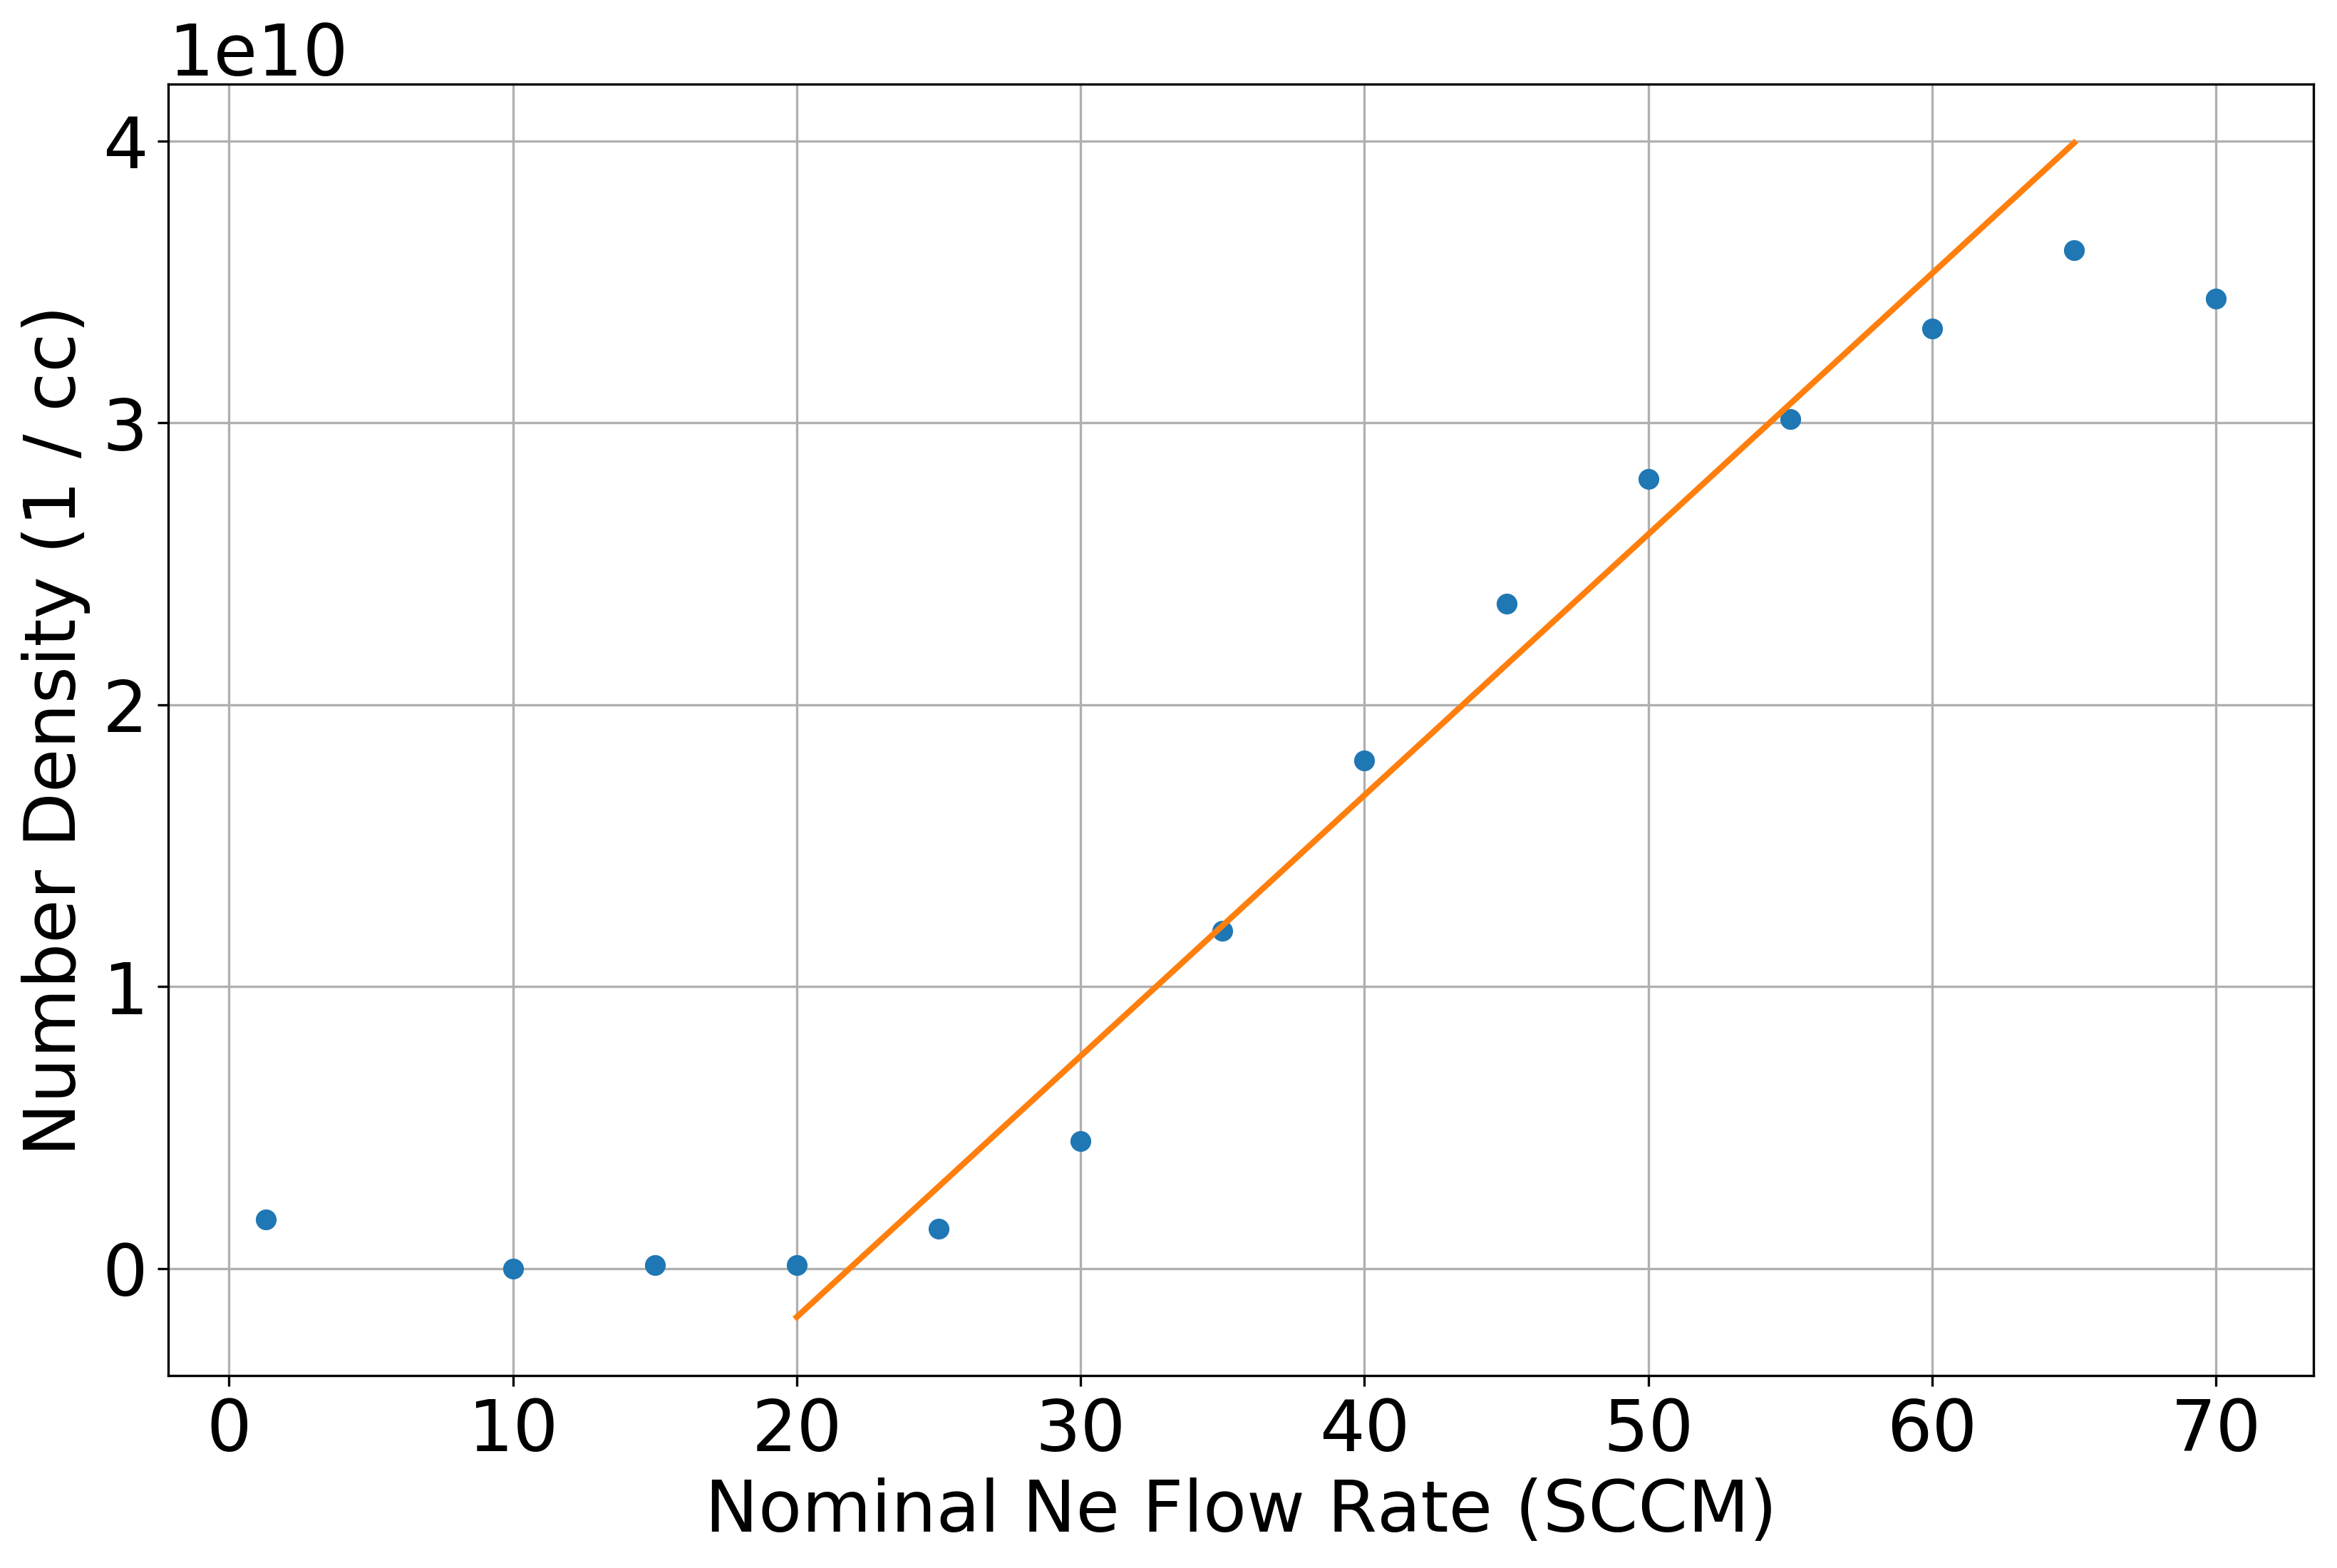
\includegraphics[width=0.8\textwidth]{images/CBGB_hydrodynamic_fit.png}
	\caption{Fitted linear behavior of \ce{H2O} entrained in a \ce{Ne} buffer gas beam 30 cm from cell aperture. The onset of hydrodynamic entrainment seems to occur around 20 SCCM up through $\sim$65 SCCM where the \ce{H2O} extracted into the beam has a clear linear dependence on flow rate.}
	\label{fig: rga entrainment}
\end{figure}

We find that theoretical calculations and experimental results agree that the onset of hydrodynamic entrainment occurs at a buffer gas flow rate of $\approx$ 20 SCCM. We can combine the results here with equations \ref{eq: mb_mean}, \ref{eq: n_b}, and \ref{eq: n(z)} to map out beam densities subject to all other possible parameters we may want to adjust, over our entire experimental apparatus. We start by scaling a combination of equations \ref{eq: n_b} and \ref{eq: n(z)} by $\alpha$, a buffer gas to target species density scaling factor.
\begin{equation*}
	n(z) = \alpha\frac{f}{A_{aperture} \bar{v}}\left(1-\frac{z}{\sqrt{z^2+a^2}}\right)
\end{equation*}
But this only holds true for the region in which the number density is linearly dependent to the buffer gas flow rate, not over all possible ranges; we've seen that the target species only behaves linearly in the hydrodynamic regime. This means that we should be equating the function of $n(z)$ with the linear fit performed on the data for the parameters the data was taken at.
\begin{equation*}
	mf+b = \alpha\frac{f}{A_{aperture, 0} \bar{v_0}}\left(1-\frac{z_0}{\sqrt{z_0^2+a_0^2}}\right) 
\end{equation*}
Where $z_0=30$ cm, being the distance of the RGA from the cell aperture, and $z=0=2$ mm, for the smallest aperture seen during the experimental run. We also define the experimental scaling factors:
\begin{align*}
	\alpha & = \frac{m}{\beta}+\frac{b}{\beta f} \\
	\beta & = \frac{1}{A_{aperture, 0} \bar{v_0}}\left(1-\frac{z_0}{\sqrt{z_0^2+a_0^2}}\right)
\end{align*}
Thus, we obtain a form that includes experimentally derived scaling factors that allows us to project the target species density over the length of the system.
\begin{equation}
	n(z) = \frac{mf+b}{A_{aperture} \bar{v} \beta}\left(1-\frac{z}{\sqrt{z^2+a^2}}\right)
	\label{eq: experimental n(z)}
\end{equation}

\begin{figure}[H]
	\centering
	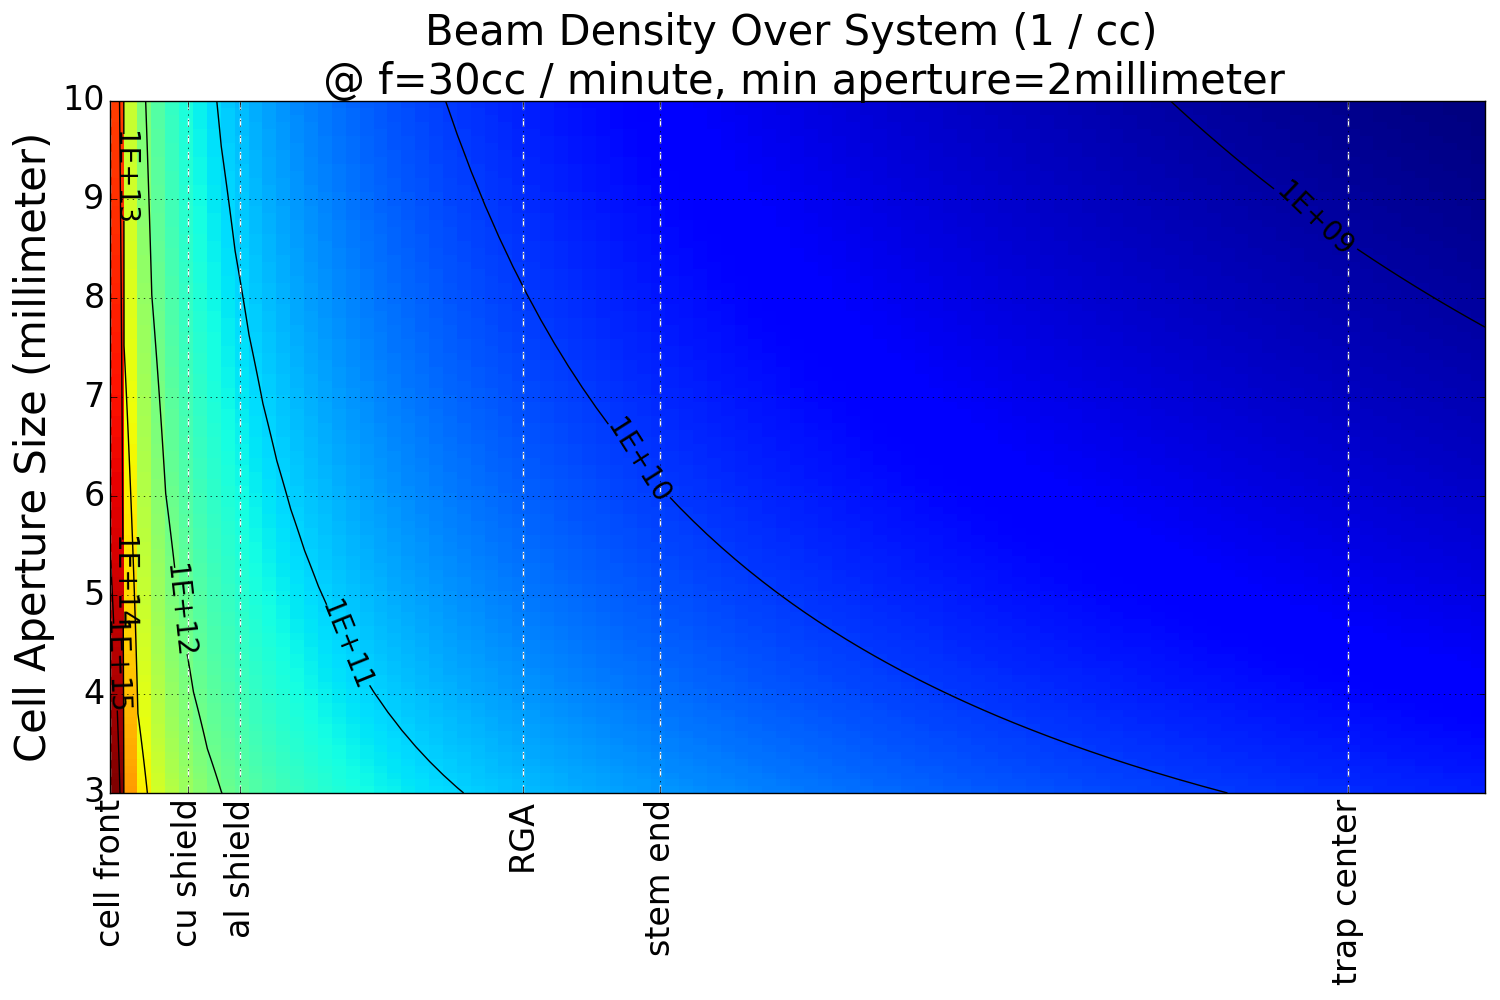
\includegraphics[width=0.8\textwidth]{images/CBGB_beam_density_over_system.png}
	\caption{Projected beam densities with a Ne flow rate of 30 SCCM with various distances of interest within the chamber. Beam densities shown are without throttling of the \ce{H2O} flow valve.}
	\label{fig: beam_density}
\end{figure}

\begin{figure}[H]
	\centering
	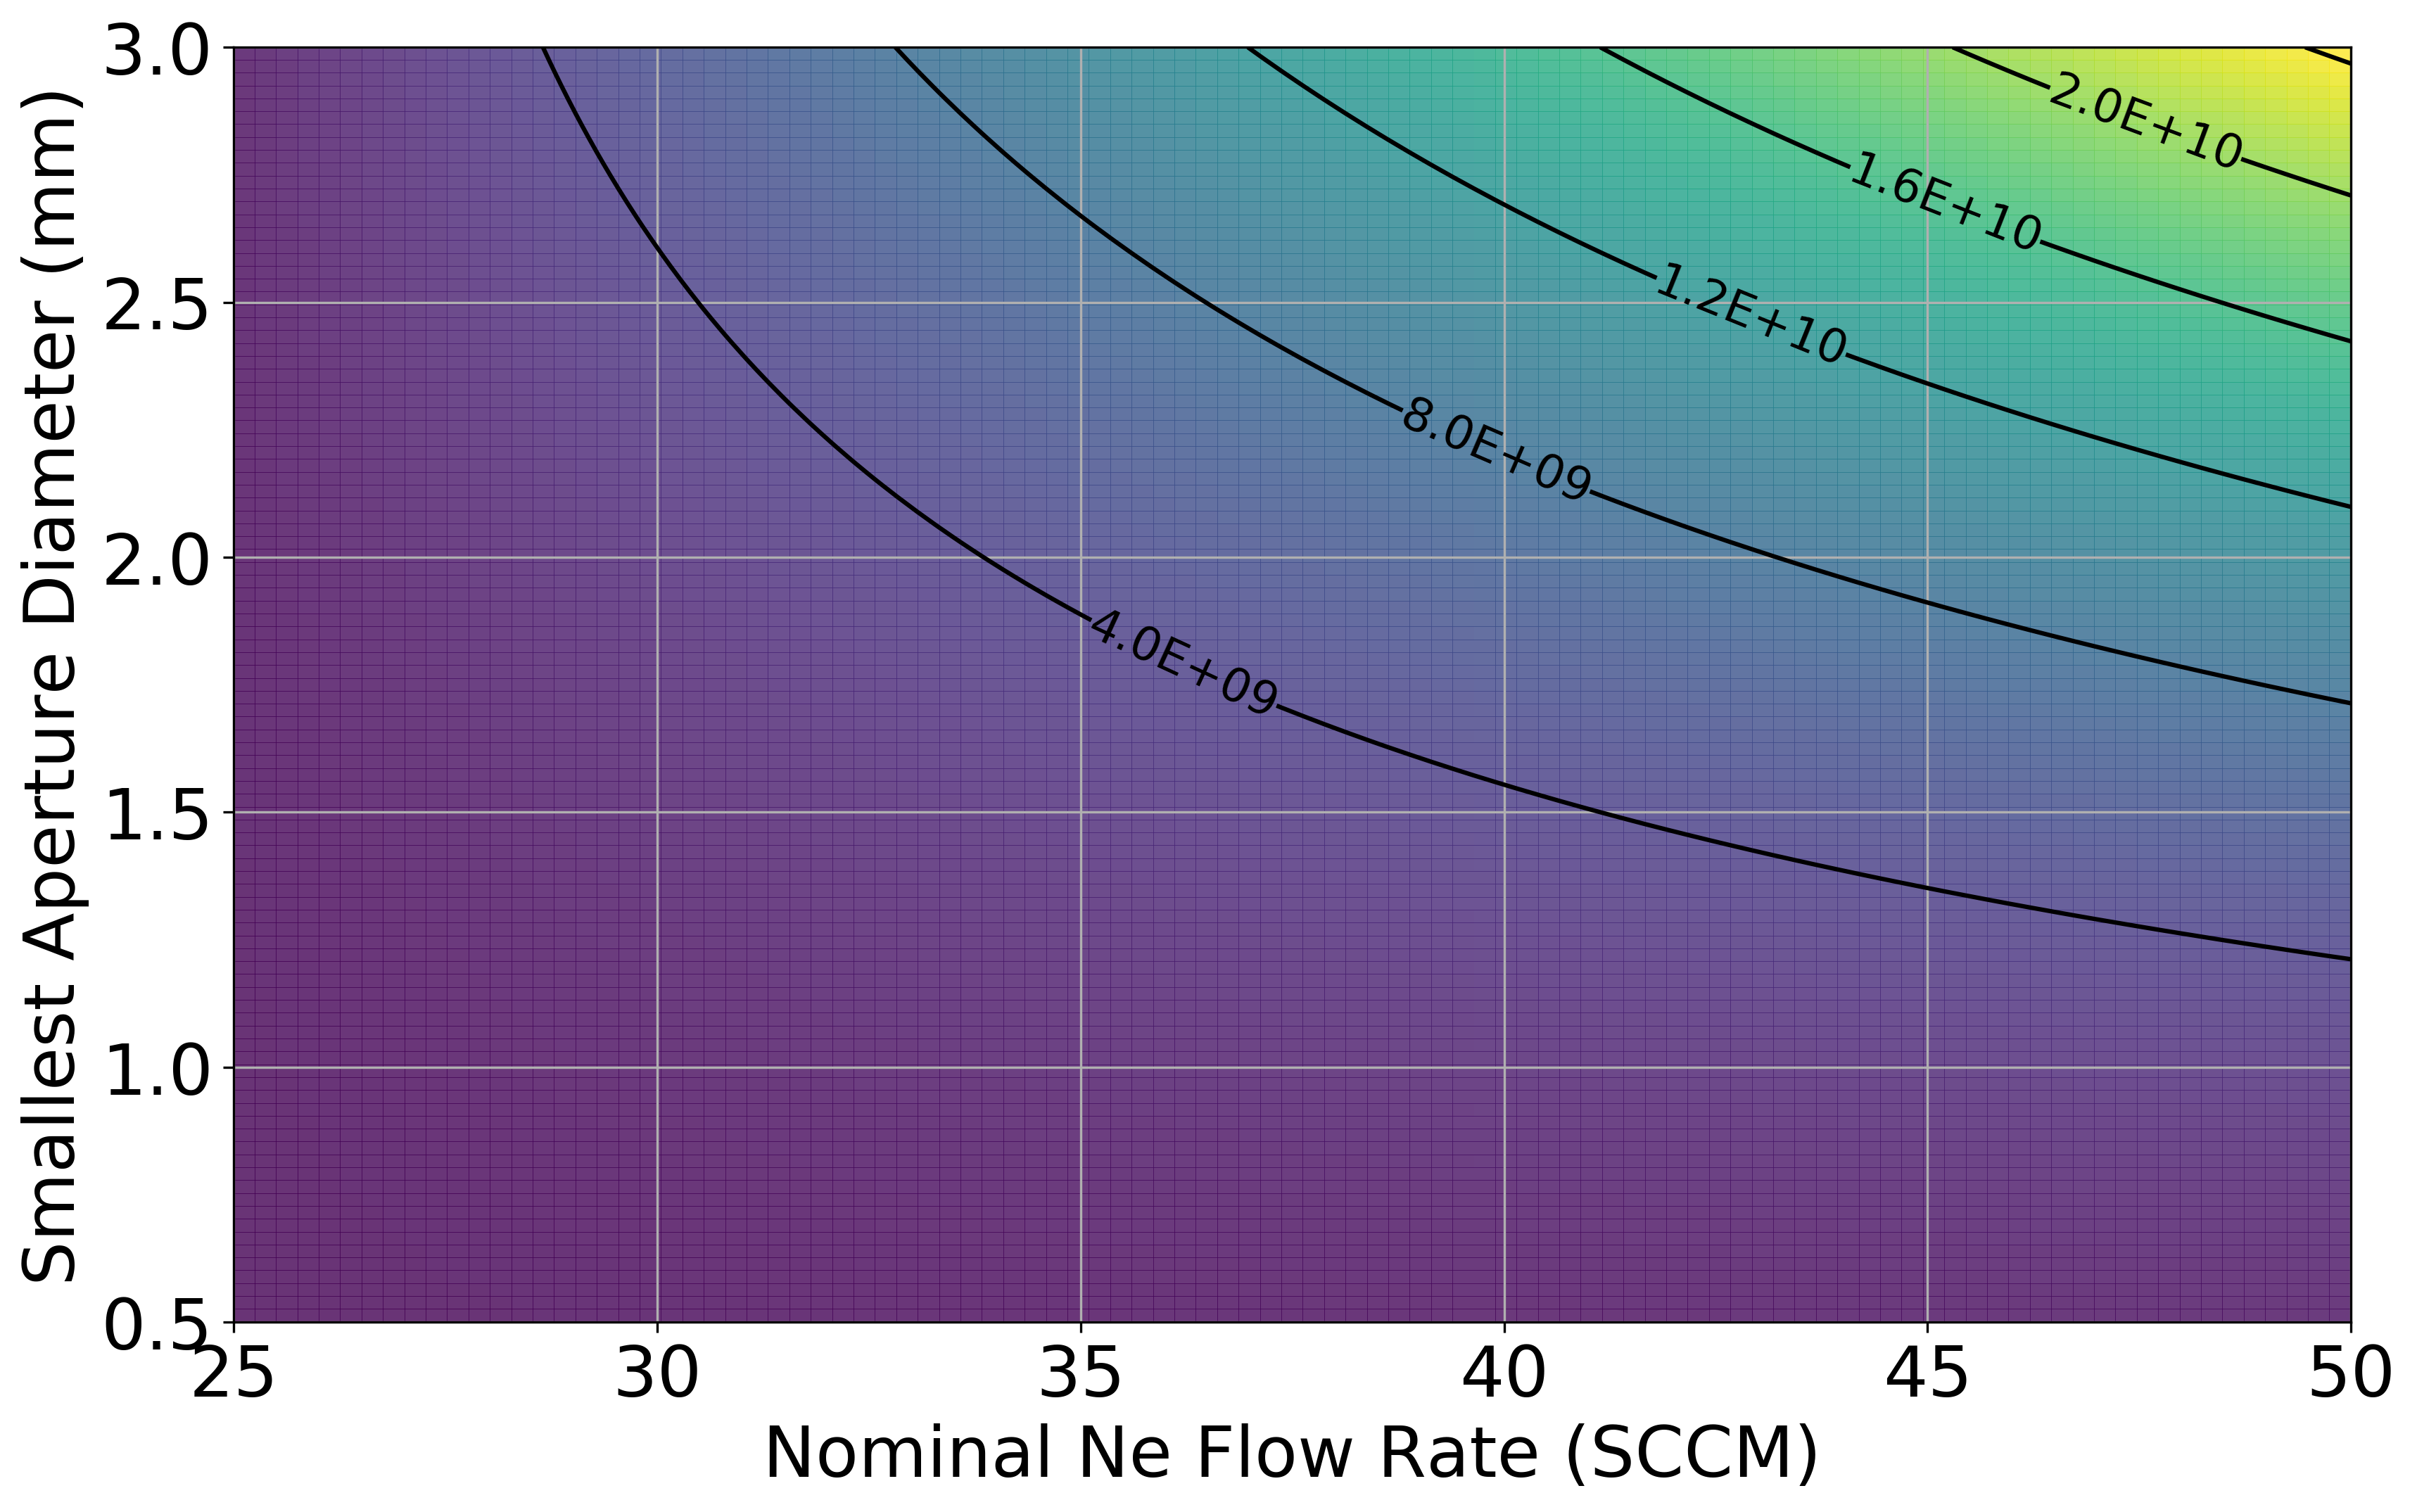
\includegraphics[width=0.8\textwidth]{images/CBGB_trap_density_aperture.png}
	\caption{Projected beam densities at the trap center over various nominal Ne flow rates and smallest skimmer aperture size. Beam densities shown are without throttling of the \ce{H2O} flow valve.}
	\label{fig: trap_density}
\end{figure}

One should not forget the mass dependence in the thermal velocity equation, which leads us to conclude that the choice of the species is a statement of the dominant species in the beam. If we choose to calculate the thermal velocity of the target species found in the beam due to the theoretical thermal velocity of the buffer gas, that indicates that the beam properties are still dominated by the buffer gas species. At target species/buffer gas ratios greater than 1/100, we may start to see the effects of the target species on not only the beam density, but also forward velocity.